\documentclass[sigconf]{acmart}
%\documentclass[conference]{IEEEtran}

\settopmatter{printacmref=false} % Removes citation information below abstract
\renewcommand\footnotetextcopyrightpermission[1]{} % removes footnote with conference information in first column
\pagestyle{plain} % removes running headers

\usepackage{algorithm}
\usepackage{algorithmic}
\usepackage{multirow}
\usepackage{colortbl}
\usepackage{dblfloatfix}
\usepackage{pifont}
\usepackage{tikz}
\usepackage{pgfplots}
\usetikzlibrary{backgrounds, positioning, fit}
\usetikzlibrary{shapes.geometric}
\usepackage{amsmath}
\usetikzlibrary{patterns}
\usetikzlibrary{pgfplots.groupplots}
\newcommand{\ballnumber}[1]{\tikz[baseline=(myanchor.base)] \node[circle,fill=.,inner sep=1pt] (myanchor) {\color{-.}\bfseries\footnotesize #1};}


\begin{document}

\title{Privacy Risks of Embedded Deep Learning}

\author{Vasisht Duddu$^1$, temp$^1$}
\affiliation{\institution{$^1$ \large inst\\ $^2$ \large temp}}
\email{vduddu@tutamail.com}

%\author{
%    \IEEEauthorblockN{Vasisht Duddu\IEEEauthorrefmark{1}, D. Vijay Rao\IEEEauthorrefmark{2}, Valentina E. Balas\IEEEauthorrefmark{3}}
%    \IEEEauthorblockA{\IEEEauthorrefmark{1}Indraprastha Institute of Information Technology, Delhi, India}
%    \IEEEauthorblockA{\IEEEauthorrefmark{2}Institute for Systems Studies and Analyses, Delhi, India}
%    \IEEEauthorblockA{\IEEEauthorrefmark{3}Aurel Vlaicu University of Arad, Arad, Romania}
%    \IEEEauthorblockA{vduddu@tutamail.com, vijayrao@issa.drdo.in, valentina.balas@uav.ro}
%}



\begin{abstract}
Low powered devices demand on-device processing algorithms to meet the memory, power-efficiency and computational constraints.
In order to bring the high performing Neural Networks to edge devices, several state of the art optimizations such as model compression through \textit{pruning}, \textit{quantization}, and careful \textit{design of efficient architectures} have been extensively adopted.
These algorithms face efficiency-accuracy trade-off, but when deployed to real world sensitive applications, such as healthcare monitoring wearables, requires design for efficiency within the constraints of privacy leakage.
In this work, the three-dimensional \textit{privacy-accuracy-efficiency} tradeoff for Deep Neural Networks is addressed by evaluating the privacy risks against inference attacks on state of the art efficiency oriented Deep Learning techniques.
This privacy leakage is quantified using membership inference attacks where the adversary aims to infer whether a given data point was a member of the training data or not.
This work indicates that while stand-alone pruning reduces inference accuracy, \textit{pruning followed by retraining} (NeurIPS'15) and increasing \textit{sparsity} to the model parameters leaks more training data information.
On the other hand, aggressive quantization of Neural Network's parameters and activations lowers the membership inference risk, however, at the cost of utility.
Based on these observations, two empirical defenses: \textit{Privacy Aware Pruning} and \textit{Distilled Quantization} have been proposed that mitigate membership privacy risks \textit{while ensuring efficiency constraints}.
Further, this work extends the understanding of membership inference attacks beyond overfitting and indicates the influence of model capacity and parameter distribution.
where we explicitly add efficiency of private inference computation as a design objective of deep learning.  We use the inference-time overhead of Neural Networks as a criterion for the selection of the architecture and parameters of a model.  Given the flexibility of modifying a model during training, we can find accurate models that are also efficient for private computation.

\end{abstract}
\keywords{Membership Privacy, Inference Attacks, Efficient Deep Learning, Edge Computing.}

\maketitle




\section{Introduction}\label{introduction}

The tremendous performance of Machine Learning, especially Deep Learning, models has resulted in their deployment to low-powered edge devices and embedded systems.
Specifically, Internet of Things (IoT) devices extensively prefer on-device processing to reduce communication latency and overhead, while also preserving the privacy of data from an untrusted data curator~\cite{8110880}.
The design of efficient Neural Networks (NNs) requires algorithm-hardware co-design such as model compression, quantization, and designing special architectures with higher efficiency~\cite{8114708}.
% that are extensively used for industry applications
Such NN architecture design optimizations should conform to efficiency constraints on memory, energy, and computation overhead on embedded devices, and also maintain high prediction accuracy.
However, such designs often result in \textit{efficiency-accuracy} trade-off~\cite{rastegari2016xnornet}.

Additionally, privacy laws, such as HIPAA and GDPR, require on-device processing to maintain the privacy of user's sensitive data (e.g, medical records, location traces, and purchase preferences).
In this work we focus on Membership Inference Attack~\cite{shokri2017membership}, where given a target model and a target record, the adversary determines if the target data record was part of the target model's training data by analyzing the target model's output predictions.
For instance, wearable devices, which monitor its user's health, commonly rely on NNs for various health related predicts. Such devices are continuously trained on the private data of a large number of users, and therefore, by mounting membership inference attacks on target device, an adversary can determine if the data of a target user was used to train NNs on the target device.
In such cases, it is crucial to design NNs resistant to inference attacks, where the adversary infers unobservable, sensitive information (e.g, user's health status) from the observable information (e.g., model predictions).
We refer to computations that achieve privacy through inference-resistance as {\em privacy-preserving computation}.
%Multiple works propose privacy preserving mechanisms to address the issue of privacy leakage
Such privacy preserving computation mechanisms affect the model's predictive accuracy resulting in \textit{privacy-accuracy} trade-off~\cite{Abadi:2016:DLD:2976749.2978318,DBLP:conf/ccs/NasrSH18,shejwalkar2019reconciling}.

Considering the trade-offs described above, the three objectives to consider while designing NNs for embedded devices are: (a) high prediction accuracy, (b) efficiency constraints on memory, energy, and computation overhead, and (c) preserving privacy of on-device data.
However, designing a model to preserve privacy while satisfying efficiency requirements without a significant cost of the model’s predictive accuracy is challenging.
%Designing NNs that meet all of the above objectives is a significantly challenging task due to the aforementioned trade-offs.
%In this work, we address the research question: \textit{How can we redesign NNs to reconcile privacy and efficiency in Deep NNs without a significant loss in accuracy?}

In this paper, we address this challenge by proposing \method\hspace{0.02in} — a two phase training methodology for designing NNs optimized specifically for performance, accuracy and privacy. We evaluate the privacy leakage of three state of the art hardware software co-design techniques, namely, model compression, quantization and efficient off-the shelf architectures. We show that model compression leaks more information compared to baseline (uncompressed) models indicating a higher privacy risk to the user’s data while off-the-shelf architectures (MobileNet and SqueezeNet) do not meet all the efficiency requirements but can provide limited privacy leakage. These observations motivate our design choice of quantizing NNs as part of \method\hspace{0.02in} training algorithm.

%In this paper, we first highlight the three-way trade-off between accuracy, efficiency, and privacy due to NNs designed for embedded devices.
%More specifically, we evaluate membership privacy leakage due to the three state-of-the-art hardware-software co-design techniques: model compression, quantization, and efficient off-the shelf architectures.
%We show that model compression leaks more information compared to the baseline (uncompressed) models and poses higher privacy risks to the user's data.\virat{add some numbers here}
%\red{Off-the-shelf architectures (e.g., MobileNet and SqueezeNet) do not meet all the efficiency requirements but can provide more limited privacy leakage.}\virat{clarify using numbers}
%These observations motivate our design choice of quantizing NNs as part of \method\hspace{0.02in} training algorithm.
%It is worth noting that, previous works have explored the the efficiency-accuracy~\cite{rastegari2016xnornet} and privacy-accuracy~\cite{shokri2017membership} trade-offs, however separately. To address the above shortcoming, 

% \noindent\textbf{Our contributions:} In this paper, we address this challenge by proposing %provide directions to design NNs for efficiency private inference.
% %We present 
% \method~ --- a two phase training methodology to design NNs optimized specifically for accuracy, efficiency, and privacy.
% We evaluate the privacy leakage of three state of the art hardware software co-design techniques, namely, model compression, quantization and efficient off-the shelf architectures.
% We show that model compression leaks more information compared to baseline (uncompressed) models indicating a higher privacy risk to the user's data while off-the-shelf architectures (MobileNet and SqueezeNet) do not meet all the efficiency requirements but can provide more limited privacy leakage.
% %acceptable 
% % this term should be avoided (what is acceptable?)
% These observations motivate our design choice of quantizing NNs as part of \method\hspace{0.02in} training algorithm.

%we propose \method\textemdash a two phased training methodology to design NNs optimized specifically for accuracy, efficiency, and privacy. 
In Phase-I of \method, the model parameters and activations are binarized, i.e., constrained to \{-1,+1\} to reduce the memory, energy consumption, and computation overhead.
To ensure computation efficiency, we replace the expensive multiply accumulate operations between parameter matrices and activation vectors 
% from previous layers 
to simple and cheaper XNOR operations.
As our main contribution, we show that aggressively quantized NN architectures obtained in Phase-I ensure efficient privacy-preserving computation with higher resistance to membership inference attacks.%\red{why is it better?}
Phase-I of \method\hspace{0.02in} optimizes for efficiency \textit{and} privacy but at the cost of a significant drop in accuracy.
In Phase-II, we restore this accuracy 
%to acceptable standard compared to the original (full precision model) accuracy
by transferring knowledge from larger full precision models to the quantized models~\cite{shejwalkar2019reconciling}.
Here, the quantized XNOR model uses the output predictions of the full precision state of the art models as labels instead of using the true labels during training.
This results in significantly increase in the prediction accuracy of the model while limiting privacy leakage. 
%with a small but acceptable increase in privacy leakage.

%In summary, \method\hspace{0.02in} training algorithm comprises of Phase I of \textit{Quantizing} to reduce the precision of model with binary values with XNOR computations which provides efficiency and privacy.
%This is followed by Phase II of \textit{Distillation} to restore the accuracy degradation by transferring the knowledge learnt from the full precision to the efficient quantized model.

Finally, we compare the models trained using \method\hspace{0.02in} with prior state-of-the-art defences against membership inference attacks, namely, Adversarial Regularization~\cite{DBLP:conf/ccs/NasrSH18} and Differential Privacy~\cite{Abadi:2016:DLD:2976749.2978318}.
We show that our proposed models improve the trade-offs between the efficiency,  accuracy, and privacy compared to the baselines approaches. Our work provides the first systematic evaluation efficiency-accuracy-privacy trade-offs to design a novel training methodology. The code is made publicly available\footnote{Anonymized for Submission}.
%, and show that our proposed models performance is comparable to the state of the art.
%However, our models provide an additional guarantee of higher efficiency which models trained with prior defences fail to provide.

The paper is outlined as follows: Section~\ref{background} presents background in embedded Deep Learning while Section~\ref{analysis} reports a comparative analysis of state of the art baselines.
We describe \method\hspace{0.02in} in Section~\ref{design} and evaluate it Section~\ref{compare}. Related work are then presented Section~\ref{related} before concluding in Section ~\ref{conclusions}.

%The paper is outlined as follows: We describe the threat model and describe the state of the art algorithms for embedded Deep Learning in Section~\ref{background} followed by identifying the best optimization technique to satisfy privacy and efficiency in Section~\ref{motivate}. Based on the observations, we describe the Phase I and Phase II design of \method\hspace{0.02in} training algorithm in Section~\ref{design}.
%Finally, we show that the proposed optimization for NNs is comparable to prior state of the art privacy preserving defences (Section~\ref{compare}) while additionally providing efficiency guarantees.

\section{Designing Energy Efficient Neural Networks}\label{algoback}

While DNNs deliver the state of the art accuracy on many AI tasks, it comes at the cost of high computational complexity.
Therefore, the progress in Deep learning is limited by how fast the NNs can be computed.
For real time applications, it requires low latency inference where small number of images can be classified quickly.
However, we cannot rely on processing manufacturing companies to provide better CPUs as Moore's law is no longer providing extra computation.
Accordingly, techniques that enable efficient processing of DNNs to improve energy efficiency and throughput without sacrificing the application accuracy or increasing hardware cost are critical to the wide deployment of DnNs in AI systems.




Training and Inference Efficiency:
The storage requirements are higher to store the intermediary values and output of backprop; Precision required for rtaining training is higher than precision required for inference.
While there are some techniques to improve the efficiency of training, we focus only on improving the efficiency of prediction stage.Computation requirement for training and inference vary where training requires powerful resources taking days and multiple hours in the cloud.
While inference can be performed locally on the edge(IoT or mobile).
In many applications, it is desirable to have computation near the sensors (edge computing) to reduce the commnication latency and cost and lowering the security risks of processing senstitive data on the cloud.
However, many of the embedded devices on the edge have stringent energy conumption, computation and memory limitations requiring efficient processing of NNs.
The key metrics for embedded machine learning include accuracy (utility), energy consumption, throughput and cost.

Energy consumption is often dominated by data movemet as memory access consumes singificantly more energy than computation[M Horowitz: COmputing's energy problem and what we can do about it]
The cost is dictated by the memory consumption or storage required on the chip.
Throughput which is dictated by the amount of computation and increases with the dimensionality of the data.

While specialised hardware addresses these issues fby optimising the data flow, minimising access to expensive levels of memeory and reuse at lower levels of memroy hierarcy[cite eyeriss paper], we only consider the joint algorith-hardware co-design techniques which aim to optimise the NNs for embedded devices.

In this work, we investigate the problem of performing privacy-preserving inference on neural networks. Let $\theta$ be the model parameters stored on the server, $x$ be the client's input, $y$ be the expected output and $f$ is the inference function to be computed. Given this, we want to compute the below function:

\begin{equation}
f(x,\theta)\rightarrow y
\end{equation}


\paragraph{Parameter.}
As our first observation, we present that the number of gates can be calculated as a function of the parameter size in the network. Thus, smaller parameter values result in lower of number gates to represent them. Table~\ref{tbl:gc_complexity} shows the number of total gates, non-XOR gates and communication required to design circuits for basic operations such as addition, multiplicaiton, greater than and so on. We observe that inputs with lesser bit sizes require smaller number of non-XOR gates, thereby exhibiting efficienct execution performance. Moreover, the number of bytes communicated are directly proportional to the
input size as well.

Neural networks have shown to exhibit high accuracies even with 8-bit or 16-bit precision and do not need to have 32 or 64-bit precision. Ideally, the lowest possible value that a parameter can take is 1 bit. Binary neural networks have achieved accuracies almost similar to those of standard networks for dataset such as MNIST, CIFAR and others.  This naturally aligns with our selected cryptographic primitive as each wire in garbled circuits represents 1 bit value.  Binarizing the model parameters further allows us to heavily use the free XOR, XNOR and NOT gates in garbled circuits. We present detailed information regarding the construction in Section~\cite{}.
Based on this observation, we propose the first optimization of reducing the parameter sizes. We reduce the parameter sizes in the network to design smaller garbled circuits while retaining the accuracy of the original model.

In this paper, we aim to answer the following research question:

{\em Whether it is possible to redesign neural network algorithms for secure computation while achieving acceptable accuracy and efficiency simultaneously?}

\paragraph{Structures.}
Next, we observe that the structure of the neural network itself heavily influences the number of gates in the circuit. Designing optimized circuits depends on several factors in the network architecture such as the number of layers in the network, number of neurons per layer, the connections between them and so on. For example, varying the number of kernels, stride size, padding  for convolutional layers directly affects the computation and communication cost of garbled circuits.
Further, we observe that deeper networks having small number of inputs at each layer are better suited for GC. We utilize these observations to modify the structure of neural networks while retaining inference accuracy comparable to standard models.

In designing our solution, we aim for the following main goals:

\begin{itemize}
\item {\em Privacy-}
The solution should preserve privacy of the model parameters $\theta$ from the users and that of $x$ and $y$ from the server.

\item {\em Accuracy-}
The drop in accuracy of the privately computed inference function should be minimum as compared to the accuracy of the model on plaintext data.

\item {\em Performance-}
The private computation should demonstrate acceptable performance overhead, preferably within a few milliseconds per inference request.

\end{itemize}


add section for energy efficiency for each of the efficient training algorithms.

Instead of using multiplication and addition circuits, we perform XNOR operations on the inputs followed by a bitcount operation. This reduces the overall number of non-XOR gates used to compute the operation. The equation can be represented as follows.

\begin{align}
\mathbf{x} \cdot \mathbf{w} =
N - 2\times\operatorname{bitcount}(\operatorname{xnor}(\mathbf{x}, \mathbf{w}))
\end{align}

As our main contribution, we show that neural network algorithms can be heavily optimized to execute efficiently using garbled circuits. We observe that the efficiency of evaluating an inference circuit depends on two key factors: the model parameters and the network structure.  With this observation,  selects optimal parameter size and network structure to guarantee acceptable {\em performance}. Last but not the least, to ensure high {\em accuracy} of the model,  uses an architecture search approach to find the best model with high accuracy and efficiency on garbled circuits.

In this paper, we provide directions to design neural networks for secure inference and low private computation overhead. We show that our optimized neural network architectures execute faster than Gazelle, the most efficient existing solution on privacy-preserving deep learning inference.


\pgfmathdeclarefunction{gauss}{2}{%
  \pgfmathparse{1/(#2*sqrt(2*pi))*exp(-((x-#1)^2)/(2*#2^2))}%
}


\begin{figure*}[ht!]
\begin{center}% note that \centering uses less vspace...
\resizebox{2\columnwidth}{!}{%
\begin{tabular}{lllll}


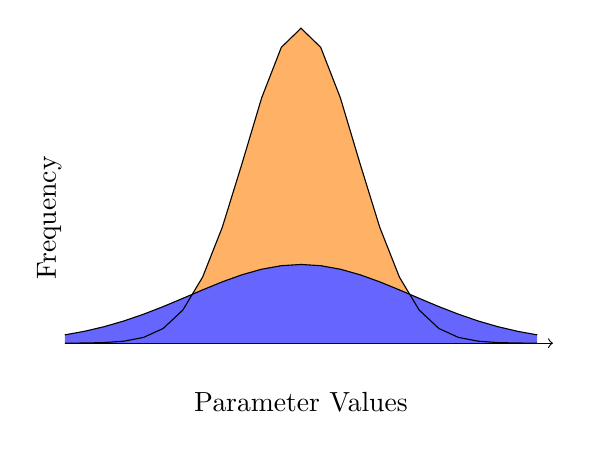
\begin{tikzpicture}
% define normal distribution function 'normaltwo'
\def\normaltwo{\x,{4*1/exp(((\x-3)^2))}}
\def\normal{\x,{1/exp(((\x-3)^2)/(4))}}


% Shade orange area underneath curve.
\fill [fill=orange!60] (0,0) -- plot[domain=0:6] (\normaltwo) -- (6,0) -- cycle;
\fill [fill=blue!60] (0,0) -- plot[domain=0:6] (\normal) -- (6,0) -- cycle;

% Draw and label normal distribution function
\draw[color=black,domain=0:6] plot (\normaltwo) node[right] {};
\draw[color=black,domain=0:6] plot (\normal) node[right] {};


% Optional: Add axis labels
\draw (-.2,2.5) node[left, rotate=90] {Frequency};
\draw (3,-.5) node[below] {Parameter Values};

% Optional: Add axes
\draw[->] (0,0) -- (6.2,0) node[right] {};
%\draw[->] (0,0) -- (0,5) node[above] {};

\end{tikzpicture} &


%
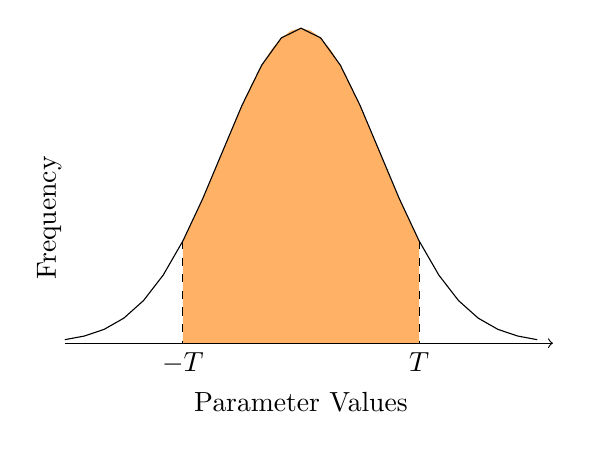
\begin{tikzpicture}
% define normal distribution function 'normaltwo'
\def\normaltwo{\x,{4*1/exp(((\x-3)^2)/2)}}

% input y parameter
\def\y{4.5}
\def\z{1.5}

% this line calculates f(y)
\def\fy{4*1/exp(((\y-3)^2)/2)}
\def\fz{4*1/exp(((\z-3)^2)/2)}

% Shade orange area underneath curve.
\fill [fill=orange!60] ({\z},0) -- plot[domain=1.5:4.5] (\normaltwo) -- ({\y},0) -- cycle;

% Draw and label normal distribution function
\draw[color=black,domain=0:6] plot (\normaltwo) node[right] {};

% Add dashed line dropping down from normal.
\draw[dashed] ({\y},{\fy}) -- ({\y},0) node[below] {$T$};
\draw[dashed] ({\z},{\fz}) -- ({\z},0) node[below] {$-T$};


% Optional: Add axis labels
\draw (-.2,2.5) node[left, rotate=90] {Frequency};
\draw (3,-.5) node[below] {Parameter Values};

% Optional: Add axes
\draw[->] (0,0) -- (6.2,0) node[right] {};
%\draw[->] (0,0) -- (0,5) node[above] {};

\end{tikzpicture} &





%
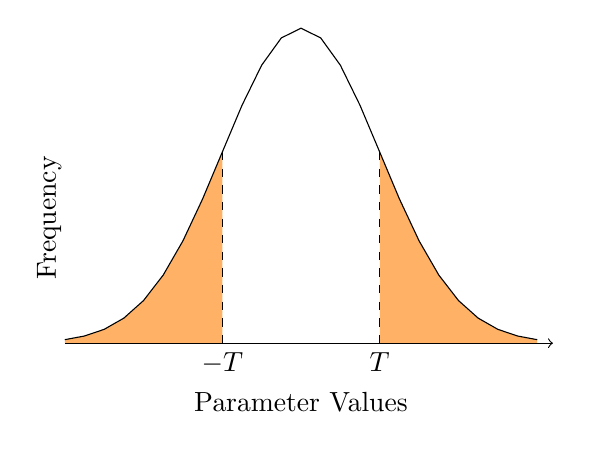
\begin{tikzpicture}
% define normal distribution function 'normaltwo'
\def\normaltwo{\x,{4*1/exp(((\x-3)^2)/2)}}

% input y parameter
\def\y{4}
\def\z{2}

% this line calculates f(y)
\def\fy{4*1/exp(((\y-3)^2)/2)}
\def\fz{4*1/exp(((\z-3)^2)/2)}

% Shade orange area underneath curve.
\fill [fill=orange!60] (0,0) -- plot[domain=0:2] (\normaltwo) -- ({\z},0)  -- cycle;
\fill [fill=orange!60] (4,0) -- plot[domain=4:6] (\normaltwo) -- (6,0)  -- cycle;

% Draw and label normal distribution function
\draw[color=black,domain=0:6] plot (\normaltwo) node[right] {};

% Add dashed line dropping down from normal.
\draw[dashed] ({\y},{\fy}) -- ({\y},0) node[below] {$T$};
\draw[dashed] ({\z},{\fz}) -- ({\z},0) node[below] {$-T$};


% Optional: Add axis labels
\draw (-.2,2.5) node[left,rotate=90] {Frequency};
\draw (3,-.5) node[below] {Parameter Values};

% Optional: Add axes
\draw[->] (0,0) -- (6.2,0) node[right] {};
%\draw[->] (0,0) -- (0,5) node[above] {};

\end{tikzpicture}

\end{tabular}
}
\caption{.}
\label{fig:loss}
\end{center}
\end{figure*}


\textbf{Machine and Deep Learning.}

\textit{Quantized Neural Networks}

One approach of improving efficiency for Neural Networks is through quantizing the parameter values and hence, reducing the precision of parameters number of bits required to represent the values in hardware \cite{Hubara:2017:QNN:3122009.3242044}.

A specific case of quantized Neural networks is using binary parameter and activation values\{-1,+1\} \cite{NIPS2016_6573}\cite{NIPS2015_5647}
For such binarized Neural Networks, the computation overhead due to matrix multiplication can be replaced by cheaper XNOR computation \cite{rastegari2016xnornet}\cite{DBLP:journals/corr/ZhouNZWWZ16}.
BNNs result in lower accuracy compared to full precision counterparts and several research papers and explored improving the accuracy-efficiency trade-off \cite{AAAI1714619}.
Ternary weighted Networks provide better accuracy compared to BNNs at the cost of higher precision with weights \{-W,0,+W\} where the threshold $W$ can be learned for higher performance \cite{DBLP:journals/corr/ZhuHMD16}\cite{Li2016TernaryWN}

\begin{algorithm}
\begin{algorithmic}
    \FOR{$k=1$ to $L$}
        \STATE $W_k^b \leftarrow {\rm Binarize}(W_k)$
        \STATE $a_k \leftarrow a_{k-1}^b W_k^b$
        \IF{$k < L$}
            \STATE $a_k^b \leftarrow {\rm Binarize}(a_k)$
        \ENDIF
    \ENDFOR

\end{algorithmic}
\caption{
Inference Stage of Binary Neural Network; Binarize() function is deterministic thresholding scheme; $W_k^b$ are the binarized weights($W_k$) and $a_k$ is the activation of the $k^{th}$ layer
}
\label{alg:train}
\end{algorithm}


\textit{Pruning.} \cite{Han:2015:LBW:2969239.2969366}


\textit{Efficient Architecture Design.} The design space for Neural Networks enables to find multiple models with different complexity but same accuracy.
Smaller Neural Networks allow to deploy on FPGA's and other low-powered devices with limited memory.
Two such Neural Network models are SqueezeNet \cite{DBLP:journals/corr/IandolaMAHDK16} and MobileNetV2 \cite{conf/cvpr/SandlerHZZC18} which are specifically designed to have less number of parameters and memory footprint.


\textit{Efficient Training Pipelines}

Dense sparse dense training \cite{DBLP:journals/corr/HanPNMTECTD16}
Model compression pipeline cobining pruning, quantization and huffman coding \cite{DBLP:journals/corr/HanMD15}
Huffman Coding is used for representation while storing in the hardware and in our experiments, we use pruning followed by quantization to achieve model compression.


Compact Network Architectures: The number of parameters and complexity of etwork can be optimized by careful design of the network architecture itself.
Here, instead of replacing larger filters with a set of smaller filters which have fewer weights in total when the filters are applied sequentially they have same overall receptive field.
For instance, one 5x5 filter can be replace with 2 3x3 filters. 1x1 convolutional layers can be used to reduce the number of channels in output feature map and hence the overall computation.
Forexample,32 ltersof1x1x64can transform an input with 64 channels to an output of 32 channels and reduce the number of  lter channels in the next layer to 32. SqueezeNet uses many 1 x 1  lters to aggressively reduce the number of weights [157]. It proposes a  re module that  rst “squeezes” the net- work with 1 x 1 convolution  lters and then expands it with multiple 1 x 1 and 3 x 3 convolution  lters.
It achieves an overall 50x reduction in the number of weights compared to AlexNet, while maintaining the same accuracy
Replace 3x3 filters with 1x1 filters.Given a budget of a certain number of convolutionfilters,  we will choose to ma
ecrease the number of input channels to 3x3 filters.Consider a convolution layerthat is comprised entirely of 3x3 filters. , to maintain a small total number of parametersin a CNN, it is important not only to decrease the number of 3x3 filters (see Strategy 1 above), butalso to decrease the number ofinput channelsto the 3x3 filters.  We decrease the number of inputchannels to 3x3 filters usingsqueeze layers, which we describe in the next section.
Downsample late in the network so that convolution layers have large activationmaps.In a convolutional network, each convolution layer produces an output activation map witha spatial resolution that is at least 1x1 and often much larger than 1x1.



Network Pruning: Neural Networks are generally overparameterised. Hence, a large amount of weights are redundant adn can be removed (set to zero) referred to as pruning.
Aggressive pruning, however, requires to finetune the model to ensure no loss in the accuracy. Typically, this is done by removing the least significant nodes in the network by computing a threshold using the senstitivity hyperparameter which is used to estimate the percentile of values.

\[
    f(W)=
\begin{cases}
    0, & \text{if } w\geq T\\
    0, & \text{if } w\leq -T\\
    w,  & \text{otherwise}
\end{cases}
\]

The original pruning requires the model to be retrained after pruning to restore accruacy while ensuring lower network size.
Further, computation on these sparse parameter matrices using specialized accelerators enable to avoid computation on 0's lower the computation complexity significantly and increasing the overall inference speed.
Prior work has indicated that over 80\% of the parameters can be pruned and the accuracy can be restored after retraining.

Sparsity: Sparsity reduces some of the values in the network close to zero replaces them as zero. This results in the distribution with two modes instead of a single gaussian distribution for the parameters.
The sparsity constraint ensures that the parameters in the middle are zeroed out while the parameter values near the tail end are updated.

\[
    f(W)=
\begin{cases}
    w, & \text{if } w\geq T\\
    w, & \text{if } w\leq -T\\
    0,  & \text{otherwise}
\end{cases}
\]

Sparse weights can be stored in a compressed format in the hardware using the compressed sparse row or column format which reduces the overall memory bandwidth[].
The decision on whether the computation is done is based on the parameter value which requires additional logic, i.e, replace output as zero without computation if parameter value is zero else perform the computation.
This also benefits in usage with SIMD or data parallel architectures and improves compression and reduces overall storage cost by using indices of weights with a zero values instead of actually storing zero values in the memory for each occurance.

Quantization reduces the precision of the operands while techniques such as pruning, sparsity reduce the number of model operation and model size.
Quantization maps parameters/activtions to a smaller set of quantization levels [qunaitized neural networks].
The ultimate goal is to minimize the error between the reconstructed data from hte quantized levels and the original data.
The number of quantized levels reflects the precision and ultimately the nuber of bits required to represent the data (log2(number of levels))
Reducing precision results in lower number of bits to represent the data which results in a lower storage cost (parameters) and/or computation cost (activation). less are and less energy [M Horowitz]
For instance, using kbits instead of 32 bits or 64 bits weights reduces the storage cost by 32/k or 64/k and hence, requires lower number of parameters to be read form the memory which further improves the energy efficiency by 32/kx or 64/kx.

The precision can be reduced aggresively to a single bit to get binary nets. Here, the weights  and activation are binarized during inference to take values \{-1,+1\} [binaryconnect, binarynet]. This allows to reduce the MAC operation to an XNOR however, with a singificant accuracy loss[xnor-net].
Several optimisaition have been considered to reduce the loss such as multiplying the outputs with a scaling factor to recover the dynamic range( weights become -w and w), keeping the first and last layer as 32 bit floating point precision and performing normatlisation before convolution to reduce the dynamic range of activations.
Further, hybrid and varying bit precision of weights and activations have been used in Dorefanet, HWGQnet and QNNs to reduce the qunatization loss.
Further, there are benefits for allowing weights to be zero (-w, 0, w) although this requires an additional bit per weight compared to binary weights, the sparsity can be used to reduce computation and storage cost [Ternary weight networks, trained ternary quantization].
Here, we consider two cases: uniform quanrization
Weight sharing forces several weight values to share a single value which reduces the number of unique weights in the model.
The weights are grouped using hashing function or k means algorithm and one value is assigned to each group.
A codebook is then built to map each grou of weights to its shared value. accordingly, the index to the corresponging group in the codebook is strored for each position n the filter rather than a eright value. This leads to a two step process to fetch the weights:
(a) read the group index from the weight memory and (b) using the griup index read the value of weight from the codebook or dictionary.

\section{Membership Inference Attacks}\label{inferenceback}

For a target machine learning model, the membership inferenceattacks aim to determine whether a given data point was used totrain the model or not [18,32,37,41,47,64]. The attack poses aserious privacy risk to the individuals whose data is used for modeltraining, for example in the setting of health analytics.Shokri et al. [47] design a membership inference attack methodbased on training an inference model to distinguish between pre-dictions on training set members versus non-members. To train theinference model, they introduce theshadow training technique: (1)the adversary first trains multiple “shadow models” which simulatethe behavior of the target model, (2) based on the shadow models’outputs on their own training and test examples, the adversaryobtains a labeled (member vs non-member) dataset, and (3) finallytrains the inference model as a neural network to perform mem-bership inference attack against the target model. The input to theinference model is the prediction vector of the target model on atarget data record.A simpler inference model, such as a linear classifier, can alsodistinguish significantly vulnerable members from non-members.Yeom et al. [64] suggest comparing the prediction confidence valueof a target example with a threshold (learned for example throughshadow training). Large confidence indicates membership. Theirresults show that such a simple confidence-thresholding method isreasonably effective and achieves membership inference accuracyclose to that of a complex neural network classifier learned fromshadow training.In this paper, we use this confidence-thresholding membershipinference approach in most cases. Note that when evaluating theprivacy leakage with targeted adversarial examples in Section 3.3.1and Section 5.2.5, the confidence-thresholding approach does notapply as there are multiple prediction vectors for each data point. In-stead, we follow Shokri et al. [47] to train a neural network classifierfor membership inference.

Passive adversary who can query the model and infer from the
no actively manipulation or tampering of the model parameters or inputs

\subsection{Adversary Assumptions}

In this work, we consider a weak black box adversary with no knowledge about the target model parameters.
This is typically the setting seen in many real world applications such as Machine Learning as a Service (MLaaS) where the users interact with the model through an API.
Within this adversarial setting, Shokri et al proposed a Membership Inference attacks based on "shadow model training".
Here, the adversary trains multiple models to mimic the behaviour of the target model and labels the membership of different output predictions.
These labeled output predictions are used to train the attack model which is a binary classifier predicting whether a given data point was IN or OUT of the dataset.
This attack relies on strong assumptions and requirements: dataset to train the shadow models is obtained from the same distribution as training data and the attacker has the capability to train large number of shadow models.
In this work, we utilize a weaker and more practical attack based on thresholding of confidence scores which does not require shadow model training and makes no assumption on the adversary's knowledge about the data distribution.
The inference accuracy is higher in case of shadow training is higher than the inference accuracy of the thresholding approach, however, this attack model is more practical and can be used by any weak adversary without additional computation overhead or knowledge assumptions.

Black-box.In this setting, the adversary’s observation is lim-ited to the output of the model on arbitrary inputs. For any datapointx, the attacker can only obtainf(x;W). The parametersof the modelWand the intermediate steps of the computationarenotaccessible to the attacker. This is the setting of machinelearning as a service platforms. Membership inference attacksagainst black-box models are already designed, which exploitthe statistical differences between a model’s predictions on itstraining set versus unseen data [6].

White-box.In  this  setting,  the  attacker  obtains  the  modelf(x;W)including  its  parameters  which  are  needed  for  pre-diction.  Thus,  for  any  inputx,  in  addition  to  its  output,  theattacker  can  compute  all  the  intermediate  computations  ofthe  model.  That  is,  the  adversary  can  compute  any  function
overWandxgiven  the  model.  The  most  straightforwardfunctions  are  the  outputs  of  the  hidden  layers,hi(x)on  theinputx.
For  a target  data  record(x,y),  the adversary  can  computethe  loss  of  the  modelL(f(x;W),y),  and  can  compute  thegradients  of  the  loss  with  respect  to  all  parametersWusing  a  simple  back-propagation  algorithm.  Given  the  largenumber of parameters used in deep neural networks (millionsof  parameters),  the  vector  with  such  a  significantly  largedimension  cannot  properly  generalize  over  the  training  data(which  in  many  cases  is  an  order  of  magnitude  smaller  insize).  Therefore,  the  distribution  of  the  model’s  gradients  onmembers  of  its  training  data,  versus  non-members,  is  likelyto  be  distinguishable.  This  can  help  the  adversary  to  runan  accurate  membership  inference  attack,  even  though  theclassification  model  (with  respect  to  its  predictions)  is  well-generalized.

Gradient vector over all parameters are cmbined to compute membership probability of the target data point using autoencoder with unsupervised learning and further use clustering algorithm to serparate members and non-members given membership probability as the feature vector.
Pass all the weights/gradients to the encoder to obtain single value representing the membership prob. Train the decoder to reconstruct original vector from the membership prob.

the adversary first obtains M(xTarget ). Then, she extracts the highest pos- terior and compares whether this maximum is above a certain threshold. If the answer is yes, then she predicts the data point is in the training set of the target model and vice versa. The reason we pick maximum as the feature follows the reasoning that an ML model is more confident, i.e., one posterior is much higher than others, when facing a data point that it was trained on. In another words, the maximal posterior of a member data point is much higher than the one of a non-member data point.

We use the fraction of correct membership predictions, as themetric to evaluate membership inference accuracy. We use a testsetDtestwhich does not overlap with the training set, to representnon-members. We sample a random data point (x,y) from eitherDtrainorDtestwith an equal50%probability, to test the membershipinference attack. We measure the membership inference accuracyas follows.Ainf(F,Bε,I)=Iz∈DtrainI(F,B,z)2·|Dtrain|+Iz∈Dtest1−I(F,Bε,z)2·|Dtest|,(15)where|·|measures the size of a dataset.

The membership inference accuracy evaluates the probabilitythat the adversary can guess correctly whether an input is fromtraining set or test set. Note that a random guessing strategy willlead to a50%inference accuracy. To further measure the effective-ness of our membership inference strategy, we also use the notionof membership inference advantage proposed by Yeom et al. [64],which is defined as the increase in inference accuracy over randomguessing (multiplied by2).ADVTinf=2×(Ainf−0.5)



Mtrics: Ainf for membership inference accuracy

\section{Experimental setting}
\label{setting}

We carried out an extensive evaluation of \method. %the three state of the art design techniques for efficient model computation.
%: a) Model Compression via pruning redundant parameters and nodes, b) Quantization to lower the precision of model parameters and activations, and c) Efficient off-the-shelf architectures.
%
%We show that ... In addition, we show that ...
We first describe the datasets and architectures used in this analysis (Section~\ref{datasets}) before to present the considered comparative baselines (Section~\ref{baselines}) and metrics (Section~\ref{metrics}). %Finally, we analyse efficiency Section~\ref{eval-efficiency} and privacy leakage Section~\ref{eval-leakage}.


\subsection{Datasets and Architectures}
\label{datasets}

For evaluating and comparing different efficiency algorithms, we use two standard benchmarking datasets: FashionMNIST and CIFAR10.
We train the model for 75 epochs for FashionMNIST and 100-150 epochs for CIFAR10.
%For FashionMNIST dataset we train the model for 75 epochs and for CIFAR10, we train the models for 100-150 epochs.
%These provide us with the necessary direction to choose the optimal efficiency algorithm which satisfies all the efficiency and privacy requirement as describes in Section~\ref{motivate}.

\noindent\textbf{FashionMNIST.} This dataset consists of 60,000 training examples and a test set of 10,000 examples.
Each data record is a 28$\times$28 grayscale image which is mapped to one of 10 classes consisting of fashion products such as coat, sneaker, shirt, shoes.
For this dataset, we use a modified LeNet architecture with two convolution layers followed by maxpool and dense layers: [Conv 32 (3,3), Conv 64 (3,3), Maxpool (2,2), Dense 128, Dense 10] (Architecture 1). Additionally, we use a fully connected model [512,512,512] (Architecture 2).

\noindent\textbf{CIFAR10}. This dataset is a major image classification benchmarking dataset where the data records are composed of 32$\times$32 RGB images where each record is mapped to one of 10 classes of common objects such as airplane, bird, cat, dog.
For this dataset, we use standard state of the art architectures: Network in Network (NiN), AlexNet and VGGNet.


\subsection{Comparative Baselines}
\label{baselines}

\subsubsection{NN models for embedded systems}

%In order to execute trained NN models on low powered edge devices, optimizations are required for the design of the NN architectures.
Model designers use three state of the art approaches for designing efficient NN models for embedded systems: (a) Model Compression via Pruning, (b) quantization of model parameters and activations and (c) designing standard architectures (off the shelf efficient architectures).
%In this work, we consider these three approaches as baselines for comparison and evaluation to select the choice of optimization for \method.

\begin{itemize}[leftmargin=*]

\item {\em Model Compression (Pruning).}
NNs are overparameterized, i.e, have a large number of redundant weights.
Pruning the network refers to removing these redundant weights (setting them as zero) without a degradation of model accuracy.
The pruning operation results in a model with sparse parameters for which the hardware can be designed to skip the multiplication and memory storage, improving the efficiency.
Sparse weights can be stored in a compressed format in the hardware using the compressed sparse row or column format which reduces the overall memory bandwidth~\cite{DBLP:journals/corr/HanMD15,10.1109/ISCA.2016.30,Han:2015:LBW:2969239.2969366}.
Aggressive pruning, while compressing the model significantly, requires to be re-trained to restore the model's original accuracy.
For a sensitivity threshold $T$, the parameters close to zero are replaced by zero: % which is given as:
\[
\footnotesize
    f(W)=
\begin{cases}
    0, & \text{if } -T \leq w \leq T\\
    w,  & \text{otherwise}
\end{cases}
\]

\item {\em Off-the-Shelf Efficient Architectures.}
NNs can be redesigned by changing the hyperparameters (i.e., filter size in convolution, number of layers and their types) to reduce the number of parameters and hence, the memory footprint.
One approach is to replace larger convolution filters with multiple smaller filters with less number of parameters but covering the same receptive fields.
For instance, one 5x5 filter can be replaced by two 3x3 filters.
Alternatively, 1x1 convolutional layers reduce the number of channels in output feature map, lowering the computation and number of parameters.
For instance, for an input activation of dimension 1x1x64, 32 1x1 convolutional filters downsamples the activation maps to get an output of 32 channels.
Such optimizations enable to design compact network architecture with layers having lower parameters compared to the original model, extensively adopted in MobileNet~\cite{conf/cvpr/SandlerHZZC18} and SqueezeNet~\cite{DBLP:journals/corr/IandolaMAHDK16}.


\item {\em Quantization.}
Quantization reduces the precision of the model's parameters and the intermediate activations during execution.
Quantization maps parameters and activations to a fixed set of quantization levels~\cite{Hubara:2017:QNN:3122009.3242044}.
The number of quantized levels determines the precision of the operands ($log_2(\#levels)$).
Reducing the precision of the (a) parameters lowers the storage cost of the model in memory, (b) activations lowers the computation overhead by replacing MACs with binary arithmetic and (c) reduces the energy consumption by lowering the memory accesses and increasing throughput.
Aggressively quantizing the parameters and activations to binary and ternary precision significantly improves the overall efficiency, however, at the cost of accuracy~\cite{rastegari2016xnornet}.
For instance, Binarized NNs quantize the operands to \{-1,+1\} values~\cite{NIPS2016_6573} while ternary NNs have values \{-w, 0, w\} where $w$ can be fixed or learnt during training~\cite{Li2016TernaryWN}. These are examples of uniform quantization.
Alternatively, weight sharing maps several parameters to a single value reducing the number of unique parameters~\cite{DBLP:journals/corr/HanMD15}.
%This mapping is done using K-Means clustering or a hashing function and the corresponding shared values are read from a "codebook" which maps different parameters to its shared value.
This mapping is done using K-Means clustering or a hashing function where a "codebook" maps different parameters to the corresponding shared values.

\end{itemize}


\subsubsection{Privacy defences}


%In this work,
We consider two state of the art baselines: Adversarial Regularization and Differential Privacy.
These defences have mainly focussed on improving the model's generalization and reduce overfitting which has been considered as the main cause for leakage through membership inference attacks.

\begin{itemize}[leftmargin=*]
\item {\em Adversarial Regularization (AdvReg)~\cite{DBLP:conf/ccs/NasrSH18}.} Here, the problem of defending against membership inference attack is modelled as a minimax game between two NNs: classifier network and attacker network.
The two networks are trained alternatively with conflicting objectives: first, the attacker network is trained to distinguish between the training data members and non-members followed by training the classifier network to minimize the loss as well as fool the attacker network.
Formally, the target classifier outputs a single probability $I(F(x),y) \in [0,1]$ which indicates the likelihood of $x$ being part of the training data.
The classifier minimizes the loss along with the output of the attacker classifier balanced with a privacy risk hyperparameter $\lambda$ : $min_{\theta} l(F(x),y) + \lambda log(I(F(x),y))$.

\item {\em Differential Privacy (DP)~\cite{Abadi:2016:DLD:2976749.2978318}.} In this work, we specifically consider DP-SGD which adds carefully crafted noise to the gradients during backpropagation in SGD algorithm.
The noise is sampled from a Laplacian or Gaussian distribution proportional to the model's sensitivity which is then added to the gradients during backpropagation.
This provides provable bound on the information leaked about an individual data record in the dataset and ensures that the presence or absence of a data record does not change the model's output, hence defending against membership inference attacks.
\end{itemize}

\subsection{Metrics}
\label{metrics}

\noindent\textbf{Efficiency.} We evaluate efficiency on Memory efficiency, Computation efficiency and Energy efficiency. Memory efficiency is compared based on the reduction in the memory footprint of the model computed from the parameters stored in the memory. Computation efficiency is compared based on the reduction in the MAC operations which influences the execution time. Finally, the energy consumption is compared based on memory accesses from reading inputs and writing results to the memory. Since, significant literature has compared the efficiency empirically~\cite{8114708}, we provide a qualitative comparison for the baseline algorithms.

\noindent\textbf{Privacy.} We use the inference attack accuracy to estimate the success of membership inference attack.
An accuracy above random guess $50\%$ indicates a training data leakage through membership inference attack.
This indicates that the adversary is able to identify the membership details of a data record with an accuracy higher than random guess.
The success of inference attack accuracy is strongly correlated with the model's extent of overfitting empirically measured as the difference between the train and test accuracy (i.e., generalization error). Higher generalization error (i.e., overfitting) results in higher distinguishability between the test and train resulting in higher membership inference accuracy~\cite{shokri2017membership}.
Additionally, the accuracy of the model is computed using the model's performance on unseen test data.

\section{Efficient Architecture Design}\label{stdarch}





\begin{table}[!htb]
\begin{center}
\renewcommand\arraystretch{1.5}
\fontsize{6.7pt}{6.7pt}\selectfont
\begin{tabular}{|c|c|c|c|c|c|}
\hline
\textbf{Architecture} & \textbf{Train}  & \textbf{Test}  & \textbf{Inference}  & \textbf{Parameters} & \textbf{Memory} \\
 & \textbf{Accuracy} & \textbf{Accuracy} & \textbf{Accuracy} & & \textbf{Footprint} \\
\hline
SqueezeNet & 88.21\% & 81.92\% & \cellcolor{green!25}53.07\% & 1.2M & 5 MB\\
MobileNetV2 & 97.50\% & 87.24\% & \cellcolor{green!25}55.57\% & 3.5M & 14 MB\\
\hline
AlexNet & 97.86\% & 80.34\% & \cellcolor{red!25}60.40\% & 61M & 240 MB\\
VGG11 & 99.13\% & 86.43\% & \cellcolor{red!25}58.04\% & 132M & 507 MB\\
VGG16 & 99.58\% & 88.95\% & \cellcolor{red!25}58.70\% & 138M &  528 MB\\
VGG19 & 99.09\% & 88.18\% & \cellcolor{red!25}57.85\% & 143M & 549 MB\\
\hline
\end{tabular}
\end{center}
\caption{Privacy Risks for Efficient Architectures.}
\label{stdarch}
\end{table}

\begin{figure}[hb!]
\resizebox{0.8\columnwidth}{!}{%
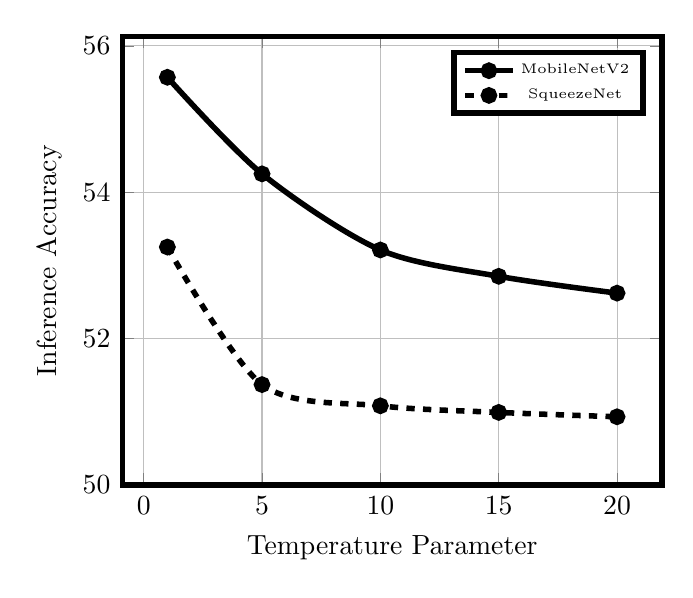
\begin{tikzpicture}
\begin{axis}[
legend style={font=\tiny},
legend pos =  north east,
line width=2.0pt,
mark size=2.0pt,
ymin=50,
legend entries={MobileNetV2, SqueezeNet},
ylabel={Inference Accuracy},
xlabel={Temperature Parameter},
% extra x ticks={1,10,...,400},
% extra y ticks={0,0.5,...,10},
% extra y tick labels={},
% extra x tick labels={},
% extra x tick style={grid=major},
% extra y tick style={grid=major},
grid=major
]
\addplot[
    color=black,
    solid,
    mark=*,
    mark options={solid},
    smooth
    ]
    coordinates {
    (1,55.57)(5,54.25)(10,53.21)(15,52.85)(20,52.62)
      };
\addplot[
      color=black,
      dashed,
      mark=*,
      mark options={solid},
      smooth
    ]
    coordinates {
    (1,53.25)(5,51.37)(10,51.08)(15,50.99)(20,50.93)
      };
\end{axis}
\end{tikzpicture}
}
\caption{Standard Effiicent Architecture Design. CIFAR10}
\end{figure}

\section{Quantization}\label{quantization}

Quantization enables to reducing precision which results in lowering the model complexity.
Unlike pruning which reduces the model capacity directly by removing unnecessary nodes, quantization discretizes both the parameters and weights during inference.
The goal is to reduce the bitwidths of the tensors during computation from 32 or 64 bit floating point resulting in a significant decrease in the memory storage requirements.
For instance, the extreme case of quantization reduces the precision to binary values, i.e, the parameters and activations (during forward pass) takes the values \{+1,-1\}.

We evaluate two majoralgorithms for quantization, namely, Quantization aware training and Post-Training Quantization.
\textit{Quantization Aware Training (QAT).}

\textit{Post-Training Quantization (PTQ).}

\begin{table}[!htb]
\begin{center}
\renewcommand\arraystretch{1.5}
\fontsize{6.7pt}{6.7pt}\selectfont
\begin{tabular}{|c|c|c|c|c|}
\hline
\multicolumn{5}{|c|}{\textbf{FashionMNIST}}\\
\hline
\textbf{Architecture} & \textbf{Memory} & \textbf{Train}  & \textbf{Test}  & \textbf{Inference}  \\
 & \textbf{Accuracy} &  \textbf{Footprint} & \textbf{Accuracy} & \textbf{Accuracy}  \\
\hline
\multicolumn{5}{|c|}{Convolutional Neural Network}\\
Full & 38.39 MB & 100\% & 92.35\% & \cellcolor{red!25}57.46\%\\
BinaryNet & 1.62 MB & 88.68\% & 86.9\% & \cellcolor{green!25}55.45\%\\
XNOR-Net & 1.62 MB & 87.19\% & 85.68\% & \cellcolor{green!25}51.05\%\\ %1,626,824 parameters
\hline
\multicolumn{5}{|c|}{Multilayer Perceptron}\\
Full & 29.83 MB & 99.34\% & 89.88\% & \cellcolor{red!25}54.86\% \\
BinaryNet & 0.93 MB & 97.61\% & 89.60\% & \cellcolor{green!25}54.30\%\\
XNOR-Net & 0.93 MB & 92.67\% & 86.68\% & \cellcolor{green!25}51.74\%\\ %937,000parameters
\hline
\hline
\multicolumn{5}{|c|}{\textbf{CIFAR10}} \\
\hline
\multicolumn{2}{|c|}{\textbf{Architecture}} & \textbf{Train}  & \textbf{Test}  & \textbf{Inference}  \\
 \multicolumn{2}{|c|}{} & \textbf{Accuracy} & \textbf{Accuracy} & \textbf{Accuracy}  \\
\hline
\multirow{2}{*}{NiN} & Full Precision & 98.16\% & 86.16\% & \cellcolor{red!25}56.69\% \\
& Binary Precision & 81.93\% & 78.74\% & \cellcolor{green!25}51.76\% \\
\hline
\multirow{2}{*}{AlexNet} & Full Precision & 97.86\% & 80.34\% & \cellcolor{red!25}60.40\% \\
& Binary Precision & 68.62\% & 66.8\% & \cellcolor{green!25}51.40\% \\
\hline
\multirow{2}{*}{VGG16} & Full Precision & 99.58\% & 88.95\% & \cellcolor{red!25}58.70\%\\
& Binary Precision & 79.67\% & 74.64\% & \cellcolor{green!25}52.65\%\\
\hline
\hline
\multicolumn{5}{|c|}{\textbf{Purchase100}} \\
\hline
\multicolumn{2}{|c|}{Full Precision} & \% & \% & \cellcolor{red!25}\% \\
\multicolumn{2}{|c|}{Binary Precision} & \% & \% & \cellcolor{green!25}\% \\
\hline
\hline
\multicolumn{5}{|c|}{\textbf{Location}} \\
\hline
\multicolumn{2}{|c|}{Full Precision} & \% & \% & \cellcolor{red!25}\% \\
\multicolumn{2}{|c|}{Binary Precision} & \% & \% & \cellcolor{green!25}\% \\
\hline
\end{tabular}
\end{center}
\caption{Privacy Risks for Low Precision Neural Networks. FashionMNIST dataset}
\label{fmnist_quantize}
\end{table}

\section{Distilled Quantization}\label{defense}

Here, we propose an apporach to reconcile membership privacy with efficient Neural Network architectures.

Distilled Quantization

\pgfdeclarelayer{background}
\pgfdeclarelayer{foreground}
\pgfsetlayers{background,main,foreground}


\tikzstyle{input} = [rectangle, rounded corners, minimum width=0.5cm, minimum height=3cm,text centered, draw=black, fill=gray!15]
\tikzstyle{layer11} = [rectangle, rounded corners, minimum width=0.25cm, minimum height=4.5cm,text centered, draw=black, fill=gray!15]
\tikzstyle{layer12} = [rectangle, rounded corners, minimum width=0.25cm, minimum height=3.5cm,text centered, draw=black, fill=gray!15]
\tikzstyle{layer13} = [rectangle, rounded corners, minimum width=0.25cm, minimum height=2.5cm,text centered, draw=black, fill=gray!15]
\tikzstyle{layer14} = [rectangle, rounded corners, minimum width=0.25cm, minimum height=1.5cm,text centered, draw=black, fill=gray!15]



\tikzstyle{input} = [rectangle, rounded corners, minimum width=0.5cm, minimum height=3cm,text centered, draw=black, fill=gray!15]
\tikzstyle{layer1} = [rectangle, rounded corners, minimum width=0.25cm, minimum height=3cm,text centered, draw=black, fill=gray!15]
\tikzstyle{layer2} = [rectangle, rounded corners, minimum width=0.25cm, minimum height=2cm,text centered, draw=black, fill=gray!15]
\tikzstyle{layer3} = [rectangle, rounded corners, minimum width=0.25cm, minimum height=1.5cm,text centered, draw=black, fill=gray!15]
\tikzstyle{layer4} = [rectangle, rounded corners, minimum width=0.25cm, minimum height=1cm,text centered, draw=black, fill=gray!15]
\tikzstyle{write} = [rectangle, rounded corners, minimum width=2.5cm, minimum height=1.5cm,text centered, draw=black, fill=gray!15]
\tikzstyle{neuron}=[circle,draw=black, fill=gray!15,minimum size=8pt,inner sep=0pt]
\tikzstyle{hidden neuron}=[neuron, draw=black, fill=gray!15]
\tikzstyle{output neuron}=[neuron, draw=black, fill=gray!15]

\begin{figure*}[!hb]
\centering
\begin{tikzpicture}[node distance=2cm, line width=1pt,every node/.style={align=center}]




\node (teach1) [layer11]  at (-9.75,0) {};
\node (teach2) [layer12]  at (-9.25,0) {};
\node (teach3) [layer13]  at (-8.75,0) {};
\node (teach4) [layer14]  at (-8.25,0) {};


\path[yshift=1.5cm, xshift=-0.5cm] node[hidden neuron] (H11) at (-7,-0.5 cm) {};
\path[yshift=1.5cm, xshift=-0.5cm]node[hidden neuron] (H12) at (-7,-1 cm) {};
\path[yshift=1.5cm, xshift=-0.5cm] node[hidden neuron] (H13) at (-7,-1.5 cm) {};
\path[yshift=1.5cm, xshift=-0.5cm]node[hidden neuron] (H14) at (-7,-2 cm) {};
\path[yshift=1.5cm, xshift=-0.5cm] node[hidden neuron] (H15) at (-7,-2.5 cm) {};

\path[yshift=1.5cm, xshift=-0.5cm] node[output neuron] (O11) at (-6.5,-1 cm) {};
\path[yshift=1.5cm, xshift=-0.5cm] node[output neuron] (O12) at (-6.5,-1.5 cm) {};
\path[yshift=1.5cm, xshift=-0.5cm] node[output neuron] (O13) at (-6.5,-2 cm) {};

\node (out1) [output neuron, right of=H13, xshift=-1cm] {};
\begin{scope}[on background layer]
    \node (teacher) [fit=(teach1) (teach2) (teach3) (teach4) (H11) (H12) (H13) (H14) (H15) (O11) (O12) (O13) (out1), fill= gray!20, rounded corners, inner sep=.2cm, label={below:Teacher Model\\(Full Precision)}] {};
\end{scope}







\node (stu1) [layer1]  at (7.5,0) {};
\node (stu2) [layer2]  at (7,0) {};
\node (stu3) [layer3]  at (6.5,0) {};
\node (stu4) [layer4]  at (6,0) {};

\path[yshift=1.5cm, xshift=-0.5cm] node[hidden neuron] (H1) at (5.75,-0.5 cm) {};
\path[yshift=1.5cm, xshift=-0.5cm]node[hidden neuron] (H2) at (5.75,-1 cm) {};
\path[yshift=1.5cm, xshift=-0.5cm] node[hidden neuron] (H3) at (5.75,-1.5 cm) {};
\path[yshift=1.5cm, xshift=-0.5cm]node[hidden neuron] (H4) at (5.75,-2 cm) {};
\path[yshift=1.5cm, xshift=-0.5cm] node[hidden neuron] (H5) at (5.75,-2.5 cm) {};

\path[yshift=1.5cm, xshift=-0.5cm] node[output neuron] (O1) at (5.25,-1 cm) {};
\path[yshift=1.5cm, xshift=-0.5cm] node[output neuron] (O2) at (5.25,-1.5 cm) {};
\path[yshift=1.5cm, xshift=-0.5cm] node[output neuron] (O3) at (5.25,-2 cm) {};

\node (out) [output neuron, left of=H3, xshift=1cm] {};
\begin{scope}[on background layer]
    \node (student) [fit=(stu1) (stu2) (stu3) (stu4) (H1) (H2) (H3) (H4) (H5) (O1) (O2) (O3) (out), fill= gray!20, rounded corners, inner sep=.2cm, label={below:Student Model\\(Binary Precision)}] {};
\end{scope}


\node (x_recon) [draw, left of=out] {$f_{student}(\mathcal{X})$};
\node (y_labels) [draw, right of=out1] {$f_{teacher}(\mathcal{X})$};

\node (classification_loss) [draw, left of=x_recon, xshift=-40] {Knowledge Distillation Loss\\$Loss_{KD}$ ($f_{student}, f_{teacher}$)};



\draw[thick,->] ([xshift=0.7cm] classification_loss.south) |- node[anchor=north, yshift=-0cm, xshift=1.5cm] {Weight Update\\(Backpropagation)} ([yshift=-1cm]student.west);
\draw[thick,->] (teacher.east) -- node[anchor=north] {} (y_labels.west);
\draw[thick,->] (y_labels.east) -- node[anchor=north] {} (classification_loss.west);
\draw[thick,->] (x_recon.west) |- node[anchor=north] {} (classification_loss.east);
\draw[thick,->] (student.west) -- node[anchor=north] {} (x_recon);

\end{tikzpicture}
\caption{\underline{\textbf{Improving the Binary Model Performance.}} The full precision model is used as a teacher model and the loss function uses the soft labels of the teacher as the target to train and update the Binary Model's performance. The resultant Binary model has a higher test accuracy trained using this fashion at the cost of a small increase in Membership Inference accuracy.}
\label{fig:advclassifier}
\end{figure*}



\begin{table}[!htb]
\begin{center}
\renewcommand\arraystretch{1.5}
\fontsize{6.7pt}{6.7pt}\selectfont
\begin{tabular}{|c|c|c|c|c|c|}
\hline
\textbf{Teacher} & \textbf{Student} & \textbf{Train}  & \textbf{Test}  & \textbf{Inference}  \\
&  & \textbf{Accuracy} & \textbf{Accuracy} & \textbf{Accuracy}  \\
\hline
Binary NiN & None & 81.93\% & 78.74\% & 51.76\% \\
Binary AlexNet & None & 68.62\% & 66.8\% & 51.40\% \\
Binary VGG16 & None & 79.67\% & 74.64\% & 52.65\%\\
\hline
NiN & Binary NiN & 90.49\% & 83.52\% & 53.90\% \\
AlexNet & Binary AlexNet & 76.79\% & 73.5\% & 51.85\% \\
VGG16 & Binary VGG16 & 89.45\% & 81.58\% & 54.98\%\\
\hline
DenseNet169 & NiN & 92.84\% & 83.71\% & 54.95\%\\
DenseNet169 & AlexNet & 81.87\% & 76.23\% & 53.51\%\\
DenseNet169 & VGG16 & 93.45\% & 85.8\% & 54.17\%\\
\hline
ResNet50 & NiN & 91.74\% & 83.77\% & 54.53\% \\
ResNet50 & AlexNet & 80.12\% & 74.92\% & 53.12\%\\
ResNet50 & VGG16 & 94.23\% & 86.52\% & 54.46\%\\
\hline
\end{tabular}
\end{center}
\caption{CIFAR10 Cross Architecture. Heterogeneous}
\label{kd}
\end{table}

\input{KDPlot_fig.tex}

\section{Pruning and Compression}\label{pruning}


Note that s is a quality parameter / sensitivity value according to the paper.
  According to Song Han's previous paper (Learning both Weights and Connections for Efficient Neural Networks),
  'The pruning threshold is chosen as a quality parameter multiplied by the standard deviation of a layer’s weights'
threshold = np.std(module.weight.data.cpu().numpy()) * s

\begin{table*}[!htb]
\begin{center}
\renewcommand\arraystretch{1.5}
\fontsize{6.7pt}{6.7pt}\selectfont
\begin{tabular}{|c|c|c|c|c|c|c|c|}
\hline
\multicolumn{8}{|c|}{\textbf{FashionMNIST Dataset}}\\
\multicolumn{2}{|c}{\textbf{Baseline Model =>}} & \multicolumn{2}{c}{\textbf{Train Accuracy:} 98.64\%} & \multicolumn{2}{c}{\textbf{Test Accuracy:} 89.66\%} & \multicolumn{2}{c|}{\textbf{Inference Accuracy:} 55.26\%}\\
\hline
\multirow{3}{*}{\textbf{Sensitivity}} & \multicolumn{4}{|c|}{On Pruning} & \multicolumn{3}{|c|}{Retraining}\\
\hline
 & \textbf{Train}  & \textbf{Test}  & \textbf{Inference}  & \textbf{Compression} & \textbf{Train}  & \textbf{Test}  & \textbf{Inference}  \\
                      & \textbf{Accuracy} & \textbf{Accuracy} & \textbf{Accuracy} & \textbf{Rate} & \textbf{Accuracy} & \textbf{Accuracy} & \textbf{Accuracy}  \\

\hline
0.25 & 98.58\% & 89.47\% & \cellcolor{green!25}55.18\% & 1.35x & 99.47\% & 89.53\% & \cellcolor{red!25}55.61\%\\
0.5 & 97.78\% & 89.17\% & \cellcolor{green!25}54.87\% & 1.87x & 99.56\% & 90.00\% & \cellcolor{red!25}55.82\%\\
0.75 & 94.97\% & 87.43\% & \cellcolor{green!25}53.86\% & 2.63x & 99.66\% & 89.56\% & \cellcolor{red!25}55.91\%\\
1 & 90.31\% & 84.45\% & \cellcolor{green!25}53.18\% & 3.76x & 99.65\% & 89.76\% & \cellcolor{red!25}55.84\%\\
1.25 & 86.68\% & 81.8\% & \cellcolor{green!25}52.46\% & 5.40x & 99.85\% & 89.73\% & \cellcolor{red!25}56.04\%\\
1.5 & 69.12\% & 65.94\% & \cellcolor{green!25}51.77\% & 7.80x & 99.75\% & 89.47\% & \cellcolor{red!25}56.04\%\\
1.75 & 49.24\% & 47.35\% & \cellcolor{green!25}51.40\% & 11.20x & 99.77\% & 89.01\% & \cellcolor{red!25}56.20\%\\
2 & 31.69\% & 30.38\% & \cellcolor{green!25}50.82\% & 15.95x & 99.89\% & 88.38\% & \cellcolor{red!25}56.69\%\\
\hline
\hline
\multicolumn{8}{|c|}{\textbf{Purchase Dataset}}\\
\multicolumn{2}{|c}{\textbf{Baseline Model =>}} & \multicolumn{2}{c}{\textbf{Train Accuracy:} 98.24\%} & \multicolumn{2}{c}{\textbf{Test Accuracy:} 88.22\%} & \multicolumn{2}{c|}{\textbf{Inference Accuracy:} 57.64\%}\\
\hline
0.25 & 98.20\% & 88.15\% & \cellcolor{green!25}57.62\% & 1.26x & 98.67\% & 87.95\% & \cellcolor{red!25}58.12\%\\
0.5 & 95.39\% & 85.37\% & \cellcolor{green!25}56.21\% & 1.65x & 99.12\% & 88.66\% & \cellcolor{red!25}58.52\%\\
0.75 & 84.78\% & 76.96\% & \cellcolor{green!25}54.04\% & 2.24x & 99.52\% & 88.94\% & \cellcolor{red!25}58.83\%\\
1 & 61.17\% & 58.04\% & \cellcolor{green!25}51.60\% & 3.13x & 99.74\% & 89.28\% & \cellcolor{red!25}59.01\%\\
1.25 & 41.22\% & 39.96\% & \cellcolor{green!25}50.81\% & 4.45x & 99.69\% & 88.51\% & \cellcolor{red!25}59.04\%\\
1.5 & 22.97\% & 22.78\% & \cellcolor{green!25}50.38\% & 6.37x & 99.89\% & 87.61\% & \cellcolor{red!25}59.71\%\\
1.75 & 15.72\% & 15.58\% & \cellcolor{green!25}50.34\% & 8.96x & 99.82\% & 85.28\% & \cellcolor{red!25}60.44\%\\
2 & 12.62\% & 12.20\% & \cellcolor{green!25}50.31\% & 12.10x & 99.64\% & 82.50\% & \cellcolor{red!25}61.05\%\\
\hline
\hline
\multicolumn{8}{|c|}{\textbf{Location Dataset}}\\
\multicolumn{2}{|c}{\textbf{Baseline Model =>}} & \multicolumn{2}{c}{\textbf{Train Accuracy:} 100.00\%} & \multicolumn{2}{c}{\textbf{Test Accuracy:} 62.3\%} & \multicolumn{2}{c|}{\textbf{Inference Accuracy:} 83.32\%}\\
\hline
0.5 & 100.00\% & 64.78\% & \cellcolor{green!25}82.54\% & 1.50x & 100\% & 64.61\% & \cellcolor{red!25}85.75\%\\
0.75 & 100.00\% & 62.70\% & \cellcolor{green!25}82.68\% & 1.94x & 100\% & 61.95\% & \cellcolor{red!25}87.69\%\\
1 & 99.96\% & 62.03\% & \cellcolor{green!25}78.76\% & 2.81x & 100\% & 62.43\% & \cellcolor{red!25}86.34\%\\
1.25 & 99.38\% & 60.39\% & \cellcolor{green!25}75.29\% & 3.43x & 100\% & 62.03\% & \cellcolor{red!25}85.25\%\\
1.5 & 95.60\% & 57.82\% & \cellcolor{green!25}70.98\% & 4.62x & 100\% & 61.15\% & \cellcolor{red!25}84.60\%\\
\hline
\end{tabular}
\end{center}
\caption{Privacy Risks for Pruning Neural Networks.}
\label{fmnist_pruning}
\end{table*}





\cite{45932}\cite{cap}
The capacity is measured using the mutual information, defined as a measure of the amount of information that one random variable contains about another random variable. The mutual information of a trained network with N input samples is calculated as follows:
\begin{equation}
I ( Y ; Y_{\theta}' | X ) = H ( Y | X ) - H ( Y | Y_{\theta}' , X )
\end{equation}
\begin{equation}
=N (1-(plog2 p+(1-p)log2 (1-p)) )
\end{equation}
where p is the mean classification accuracy for all samples under trained parameter theta. If the training accuracy is 1, the model memorizes all random samples and the I (Y ; Y' |X ) becomes the number
of samples N . If the training accuracy is 0.5, I (Y ; Y' |X ) goes to theta.
The accuracy, p, may vary depending on the training method of the model. We find N and p that maximize the mutual information of the networks by iteratively training the models.
X = \{$X_1,...,X_N$\},Xi $\in$ $(0,1)^{|N|}$
Y = $\{Y_1,...,Y_N\}$,$Y_i$ $\in$ (0,1),
Y' = $\{Y_1', ..., Y_N'\}, Y_i$' = f($\theta, X_i$),
where $f(\theta,X_i)$ is the predict of a network when the input is $X_i$. Under our experimental setting, both X and Y have uniform random distribution. Note that X and Y are independent as well as $Y_i$ and $Y_j$ when i not= j. Therefore
$P (Y_i|X_i) = P (Y_i) = 1/2$, and $H(Y) = H(Y_1, ..., Y_N ) = N H(Y_1) = N$.

And we use the network’s average accuracy p as a probability of Yi = Y'i, so that

\[
    P(Yi|Y'i)=
\begin{cases}
    p, & \text{if } Yi =Y'i\\
    (1 - p),  & \text{otherwise}
\end{cases}
\]

Finally, the equation is derived as:
\begin{equation}
I(Y;Y'|X)= H ( Y | X ) - H ( Y | Y' , X )
\end{equation}
\begin{equation}
= H ( Y ) - H ( Y | Y' ) = N -   H ( Y i | Y' i )
\end{equation}
\begin{equation}
= N -   H ( Y i | Y' i )
\end{equation}
\begin{equation}
=N-N plog2 p+(1-p)log2 (1-p)
\end{equation}
This captures
the amount of information stored in the parameters about the mapping between X and Y. To get an estimate of bits per parameter, we divide by the number of parameters,

\subsection{Sparsity vs Pruning}

We consider both the apporaches of sparsity and Pruning and evaluate their impact on membership privacy risks.
Sparsity zeros out the T\% of the parameters close to zero. In other words, the approach removes the frequently occurring parameters in the network, and forcing the model to train on the remaining network.
On the other hand, pruning ranks all the parameters and filters in a Neural Network and removes the unnecessary less occurring parameters in the network.
From the perspective of parameter distribution, pruning removes the parameters from the tail end of the distribution while sparsity removes the parameters closer to zero.

\begin{figure*}[ht!]
\begin{center}% note that \centering uses less vspace...
\resizebox{2\columnwidth}{!}{%
\begin{tabular}{lllll}


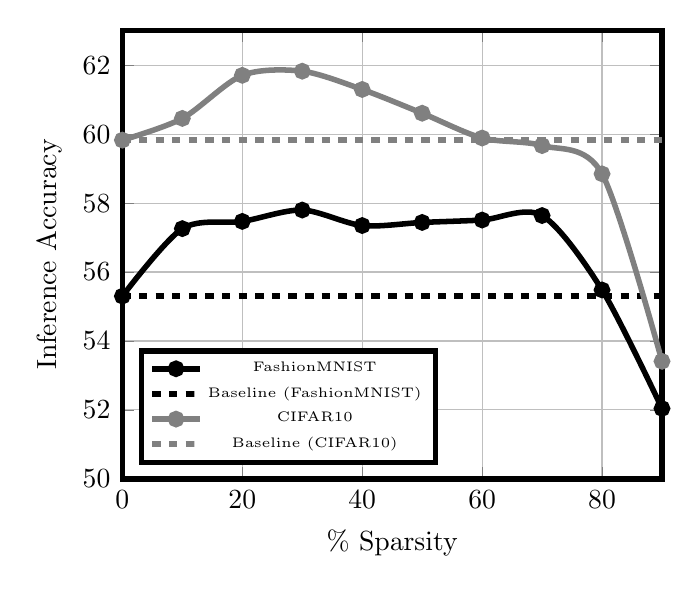
\begin{tikzpicture}
\begin{axis}[
legend style={font=\tiny},
legend pos =  south west,
line width=2.0pt,
mark size=2.0pt,
ymin=50,
xmin=0,
xmax=90,
legend entries={FashionMNIST, Baseline (FashionMNIST), CIFAR10, Baseline (CIFAR10)},
ylabel={Inference Accuracy},
xlabel={\% Sparsity},
% extra x ticks={1,10,...,400},
% extra y ticks={0,0.5,...,10},
% extra y tick labels={},
% extra x tick labels={},
% extra x tick style={grid=major},
% extra y tick style={grid=major},
grid=major
]
\addplot[
    color=black,
    solid,
    mark=*,
    mark options={solid},
    smooth
    ]
    coordinates {
    (0,55.30)(10,57.26)(20,57.47)(30,57.80)(40,57.35)(50,57.44)(60,57.51)(70,57.64)(80,55.48)(90,52.04)
      };
\addplot[
    color=black,
    dashed,
    smooth
    ]
    coordinates {
    (0,55.30)(10,55.30)(20,55.30)(30,55.30)(40,55.30)(50,55.30)(60,55.30)(70,55.30)(80,55.30)(90,55.30)
      };
\addplot[
    color=gray,
    solid,
    mark=*,
    mark options={solid},
    smooth
    ]
    coordinates {
    (0,59.83)(10,60.46)(20,61.71)(30,61.83)(40,61.30)(50,60.61)(60,59.89)(70,59.67)(80,58.85)(90,53.41)
      };
\addplot[
    color=gray,
    dashed,
    smooth
    ]
    coordinates {
    (0,59.83)(10,59.83)(20,59.83)(30,59.83)(40,59.83)(50,59.83)(60,59.83)(70,59.83)(80,59.83)(90,59.83)
      };
\end{axis}
\end{tikzpicture} &


%
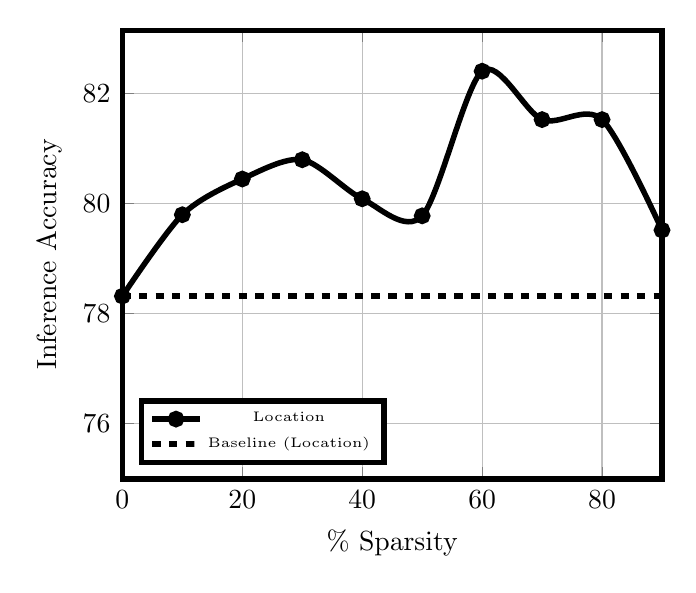
\begin{tikzpicture}
\begin{axis}[
legend style={font=\tiny},
legend pos =  south west,
line width=2.0pt,
mark size=2.0pt,
ymin=75,
xmin=0,
xmax=90,
legend entries={Location, Baseline (Location)},
ylabel={Inference Accuracy},
xlabel={\% Sparsity},
grid=major
]
\addplot[
    color=black,
    solid,
    mark=*,
    mark options={solid},
    smooth
    ]
    coordinates {
    (0,78.32)(10,79.80)(20,80.45)(30,80.80)(40,80.09)(50,79.78)(60,82.41)(70,81.53)(80,81.53)(90,79.52)
      };
\addplot[
    color=black,
    dashed,
    smooth
    ]
    coordinates {
    (0,78.32)(10,78.32)(20,78.32)(30,78.32)(40,78.32)(50,78.32)(60,78.32)(70,78.32)(80,78.32)(90,78.32)
      };

\end{axis}
\end{tikzpicture} &





%
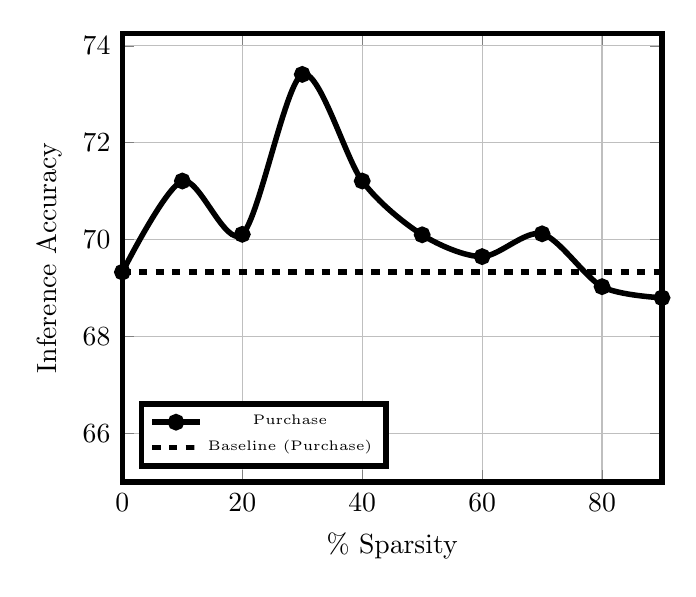
\begin{tikzpicture}
\begin{axis}[
legend style={font=\tiny},
legend pos =  south west,
line width=2.0pt,
mark size=2.0pt,
ymin=65,
xmin=0,
xmax=90,
legend entries={Purchase, Baseline (Purchase)},
ylabel={Inference Accuracy},
xlabel={\% Sparsity},
grid=major
]
\addplot[
    color=black,
    solid,
    mark=*,
    mark options={solid},
    smooth
    ]
    coordinates {
    (0,69.33)(10,71.21)(20,70.11)(30,73.41)(40,71.21)(50,70.10)(60,69.65)(70,70.12)(80,69.03)(90,68.80)
      };
\addplot[
    color=black,
    dashed,
    smooth
    ]
    coordinates {
    (0,69.33)(10,69.33)(20,69.33)(30,69.33)(40,69.33)(50,69.33)(60,69.33)(70,69.33)(80,69.33)(90,69.33)
      };

\end{axis}
\end{tikzpicture}


\end{tabular}
}
\caption{.}
\label{fig:loss}
\end{center}
\end{figure*}





\subsection{Pruning + Weight sharing}
DeepCompression
We evaluate the effectiveness of pruning followed by quantization which has been shown to have significant impact on reducing the model complexity through compression more significantly than either pruning or quantization alone.
We use the same model after pruning with Sensitivity since, it leaks the most information and evaluate the effective of quantization and whehter it can enable a good balance between test accuracy and inference accuracy.


\begin{figure*}[ht!]
\begin{center}% note that \centering uses less vspace...
\resizebox{2\columnwidth}{!}{%
\begin{tabular}{lllll}


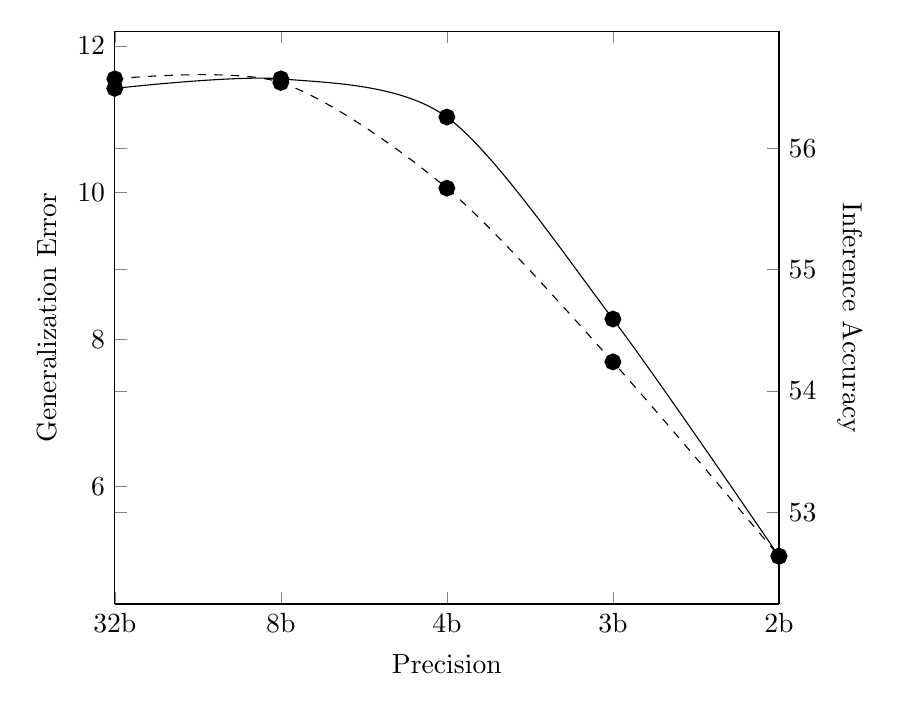
\begin{tikzpicture}
% let both axes use the same layers
\pgfplotsset{set layers}
%
\begin{axis}[
scale only axis,
line width=2.0pt,
mark size=2.0pt,
xmin=0,xmax=4,
ylabel={Generalization Error},
axis y line*=left,
xlabel={Precision},
xtick={0,1,2,3,4},
xticklabels={32b, 8b, 4b, 3b, 2b}
]
\addplot[
    color=black,
    solid,
    mark=*,
    mark options={solid},
    smooth
    ]
    coordinates {
    (0,11.42)(1,11.55)(2,11.03)(3,8.28)(4,5.05)
      };
\end{axis}

\begin{axis}[
scale only axis,
line width=2.0pt,
mark size=2.0pt,
xmin=0,xmax=4,
ylabel near ticks, yticklabel pos=right,
ylabel={Inference Accuracy},
ylabel style = {rotate=180},
axis x line=none
]
\addplot[
    color=black,
    dashed,
    mark=*,
    mark options={solid},
    smooth
    ]
    coordinates {
    (0,56.57)(1,56.54)(2,55.67)(3,54.24)(4,52.64)
        };
\end{axis}
\end{tikzpicture} &

%
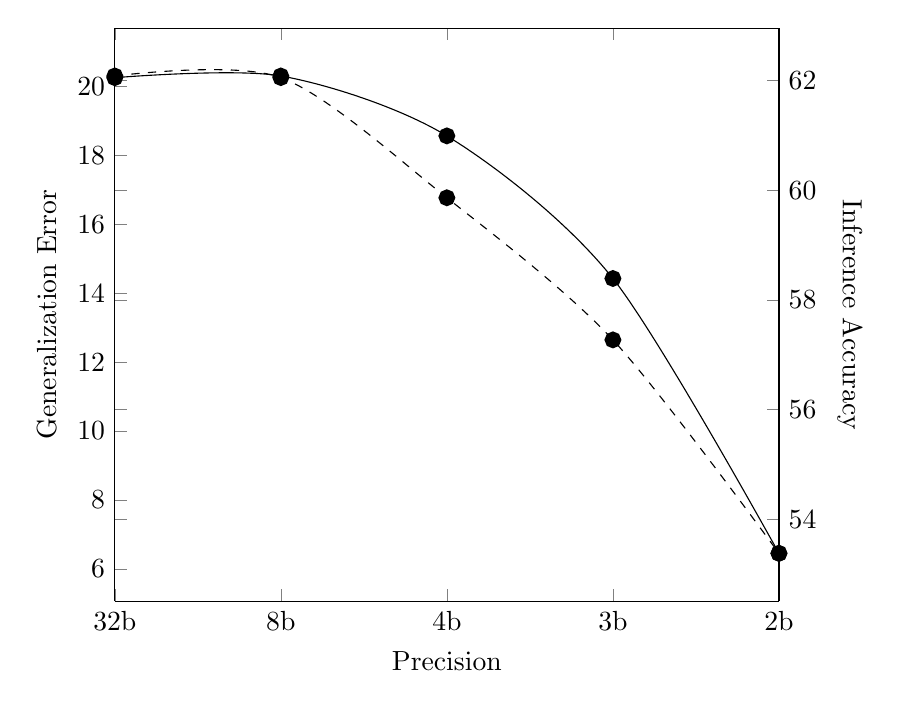
\begin{tikzpicture}
% let both axes use the same layers
\pgfplotsset{set layers}
%
\begin{axis}[
scale only axis,
line width=2.0pt,
mark size=2.0pt,
xmin=0,xmax=4,
ylabel={Generalization Error},
axis y line*=left,
xlabel={Precision},
xtick={0,1,2,3,4},
xticklabels={32b, 8b, 4b, 3b, 2b}
]
\addplot[
    color=black,
    solid,
    mark=*,
    mark options={solid},
    smooth
    ]
    coordinates {
    (0,20.26)(1,20.31)(2,18.57)(3,14.43)(4,6.45)
      };
\end{axis}

\begin{axis}[
scale only axis,
line width=2.0pt,
mark size=2.0pt,
xmin=0,xmax=4,
ylabel near ticks, yticklabel pos=right,
ylabel={Inference Accuracy},
ylabel style = {rotate=180},
axis x line=none
]
\addplot[
    color=black,
    dashed,
    mark=*,
    mark options={solid},
    smooth
    ]
    coordinates {
    (0,62.08)(1,62.05)(2,59.86)(3,57.27)(4,53.38)
        };
\end{axis}
\end{tikzpicture} &





%
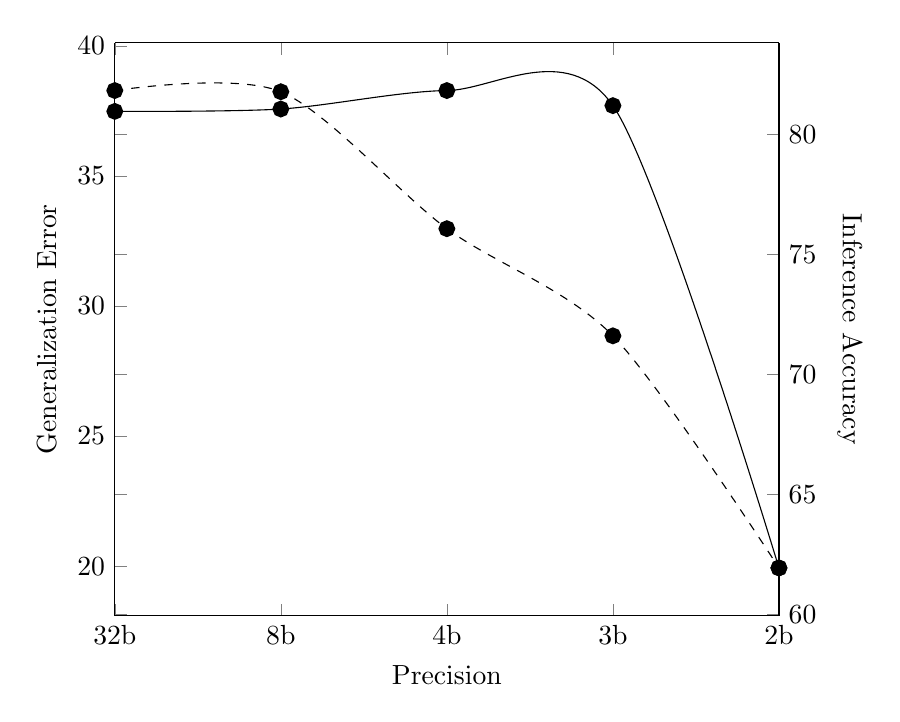
\begin{tikzpicture}
% let both axes use the same layers
\pgfplotsset{set layers}
%
\begin{axis}[
scale only axis,
line width=2.0pt,
mark size=2.0pt,
xmin=0,xmax=4,
ylabel={Generalization Error},
axis y line*=left,
xlabel={Precision},
xtick={0,1,2,3,4},
xticklabels={32b, 8b, 4b, 3b, 2b}
]
\addplot[
    color=black,
    solid,
    mark=*,
    mark options={solid},
    smooth
    ]
    coordinates {
    (0,37.48)(1,37.57)(2,38.28)(3,37.70)(4,19.93)
      };
\end{axis}

\begin{axis}[
scale only axis,
line width=2.0pt,
mark size=2.0pt,
xmin=0,xmax=4,
ylabel near ticks, yticklabel pos=right,
ylabel={Inference Accuracy},
ylabel style = {rotate=180},
axis x line=none
]
\addplot[
    color=black,
    dashed,
    mark=*,
    mark options={solid},
    smooth
    ]
    coordinates {
    (0,81.82)(1,81.77)(2,76.07)(3,71.61)(4,61.95)
        };
\end{axis}
\end{tikzpicture}


\end{tabular}
}
\caption{FashionMNIST(left) Purchase100(Center) Location(Right). Dashed is Inference accuracy, solid is generalisaton error}
\label{fig:loss}
\end{center}
\end{figure*}


\section{Privacy Aware Pruning}

To close the gap between CNN design and energy consumption optimization, we propose an privacy-aware-pruning algorithm that directly uses the membership inference accuracy of the model to guide the pruning process.
In addition, there is currently no way for researchers to estimate the inference accuracy consumption of a NN at design time.
To this extent, at each step of the pruning process, the membership inference accuracy is monitored which helps in deciding the pruning rate, i.e, how aggresively should the parameters be pruned.

We further propose a new CNN pruning algorithm with the goal to minimize overall energy consumption with marginal accuracy degradation.
We propose a new layer-by- layer pruning method that can aggressively reduce the number of non-zero weights
Instead of considering just the accuracy as a metric, we also incorporate membership privacy as an objective to be minimized while designing an efficient model.

\pgfdeclarelayer{background}
\pgfdeclarelayer{foreground}
\pgfsetlayers{background,main,foreground}


\tikzstyle{input} = [rectangle, rounded corners, minimum width=3cm, minimum height=1cm,text centered, draw=black, fill=gray!15]
\tikzstyle{arrow} = [thick,->,>=stealth]


\begin{figure}[!hb]
\centering
\begin{tikzpicture}[node distance=2cm, line width=1pt,every node/.style={align=center}]


\node (step1) [input]  at (-3,0) {\ding{202} Train Neural Network};
\node (step2) [input]  at (-3,-1.5) {\ding{203} Prune Network};
\node (step3) [input]  at (-3,-3) {\ding{204} Check Accuracy Constraint};
\node (step4) [input]  at (-3,-4.5) {\ding{205} Check Inference Constraint};
\node (step5) [input]  at (1.75,-3.75) {\ding{206} Fine Tune Network};

\begin{scope}[on background layer]
    \node (check) [fit=(step3) (step4), fill= gray!20, rounded corners, inner sep=.2cm] {};
\end{scope}


\draw [arrow] (step1.south) -- node[anchor=west] {} (step2);
\draw [arrow] (step2.south) -- node[anchor=west] {} (check.north);
\draw [arrow] (check.east) -- node[anchor=north] {No} (step5.west);
\draw [arrow] (step5.north) |- node[anchor=north] {} (step2.east);


\end{tikzpicture}
\caption{\underline{\textbf{Privacy Aware Pruning.}} Flow chart for pruning the model guided by the membership inference accuracy.}
\label{fig:advclassifier}
\end{figure}


\ballnumber{1}

The loss tolerance and the membership inference tolerance are used as constraints to the algorithm allowing the user to optimise for them while ensuring the accuracy and membership loss as required by an applicaations.
Some applications might be tolerant to accuracy loss while for other applications, even a small drop in accuracy results in a significant iimplication due to the critical nature of the application.
Similarly, some applications might forego the privacy aspect of training while for other applications, privacy is utmost crucial.
These adjustments and requirements for the application can be programmed within the algorithm to design an efficiently pruned and private model which satisfies the application requirements.

To sparsify the filters without impacting the accuracy, the simplest method is pruning weights with magnitudes smaller than a threshold, which is referred to as magnitude- based pruning [6–10]. The advantage of this approach is that it is fast, and works well when a few weights are re- moved, and thus the correlation between weights only has a minor impact on the output.

After all the layers are pruned, we fine-tune the whole network using back-propagation with the pruned weights fixed at zero. This step can be used to globally fine-tune the weights to achieve a higher accuracy. Fine-tuning the whole network is time-consuming and requires careful tuning of several hyper-parameters.

\section{Comparison with Prior Defenses}\label{compare}

Mitigating membership inference attacks has been a major research challenge requiring immediate attention.
The major reason for privacy leakage through membership inference attacks is due to overfitting in Machine Learning models.
The model performance is distinct for training data which the model has encountered previously and the unseen test data.
This difference in training and testing performance enables the adversary to train a classifier to classify a new data point into training or testing data.


\textbf{Explicit Regularization.} A straight-forward approach to mitigate membership inference attacks is to generalise the model by explicitly adding an additional regularization term.
These include Dropout, L2 penalty, model stacking (ensemble) and Knowledge Distillation.
Alternatively, a specific adversarial regularization approach that regularizes the model according to the noise
All these techniques rely on enhancing the generalisation of the model by modifying the objective function during training to reduce the difference between training and testing data.
Further, this additional regularization in the objective function results in a trade-off between utility and privacy controlled using the regularization hyperparameter.


\textbf{Provable Defenses.} Differential Privacy is a provable defense which provides a bound on the total leakage of the training data for individuals in the training data.
Particularly, Differential privacy adds noise to the gradients during training. This noise is sampled from either Gaussian and Laplacian distribution proportional to the model's sensitivity.
The current state of Differential Privacy, however, results in a privacy-utility trade-off  since adding noise to the gradients degrades the performance.
PATE framework provides a way to train model privately in a framework based on teacher-student models similar to Knowledge Distillation.
Alternatively, adding carefully crafted perturbation to the confidence scores to act as an adversarial example for the attack classifier model has also been proposed.
This approach is 


However, none of the above proposed defenses take into account the aspect of efficiency in the model design.
Such model how it impacts the deployment of models for real world applications such as wearable devices.
The proposed \textit{quantization with distillation} and \textit{privacy aware pruning} in this work, \textbf{guarantee model efficiency while mitigating privacy risks}.
We provide a comparison between the proposed defenses with the prior defenses in terms of utility and privacy loss.

\section{Related Work}\label{related}


\noindent\textbf{Machine Learning Privacy.} Data privacy in Machine Learning addresses different inference attacks such as membership inference~\cite{salem2018ml,shokri2017membership}.
While these works have been evaluated in a blackbox setting, privacy leakage through inference attacks have been studied in the context of whitebox setting~\cite{DBLP:journals/corr/abs-1812-00910}.
Further, generative model have been shown to be vulnerable to membership inference attacks~\cite{LOGANMembershipInferenceAttacksAgainstGenerativeModels} and distributed setting such as in federated learning have also been exploited~\cite{melis2019exploiting,DBLP:journals/corr/abs-1812-00910}.
These privacy leakage in machine learning models have been mainly attributed to the memorization of training data by the models~\cite{236216,10.1145/3133956.3134077}.
In order to mitigate against inference attacks several defences have been explored such as Differential Privacy~\cite{Abadi:2016:DLD:2976749.2978318}, simple and adversarial regularization~\cite{DBLP:conf/ccs/NasrSH18,salem2018ml} which aim to generalize the model and alternatively, adding noise to the predictions to increase error~\cite{10.1145/3319535.3363201}.
Alternatively, confidential computing aims to privately and efficiently compute machine learning models using secure multiparty computation~\cite{235489}.


\noindent\textbf{Efficient Deep Learning.} Hardware-Software Co-Design is crucial to accelerate the performance of NNs on hardware.
Hardware accelerators reuse weights and intermediate computation enable significant performance improvement~\cite{10.1109/ISCA.2016.30}.
Algorithmic optimizations have explored model compression through pruning~\cite{Han:2015:LBW:2969239.2969366} and reducing the precision of the model parameters and activations to binary~\cite{NIPS2016_6573}, ternary~\cite{Li2016TernaryWN} and generic quantization~\cite{Hubara:2017:QNN:3122009.3242044}.
Binarization enables to replace multiplication with simple boolean logic improving the overall performance~\cite{rastegari2016xnornet}.
Alternatively, hardware optimizations have enabled to design NN accelerators for low precision NNs for further efficiency~\cite{Umuroglu2017FINNAF}.
Further, specialized architectures designed for low memory footprint have also been extensively used for low powered devices such as mobile phones and micro-controllers~\cite{DBLP:journals/corr/IandolaMAHDK16,conf/cvpr/SandlerHZZC18}. 

\section{Conclusions}\label{conclusions}

On device processing of sensitive data using NNs on embedded systems requires a careful analysis of privacy, efficiency and accuracy of the algorithms which is currently lacking in literature.
In this work, we propose a two phase \method\hspace{0.02in} framework to design private, efficient and accurate NNs for execution on low powered embedded devices.
We quantify the privacy leakage using membership inference attacks where the adversary aims to infer whether a given data record was used in the model's training data.
We first provide a comprehensive privacy and efficiency analysis of state of the art algorithms for improving efficiency: model compression (pruning), quantization and efficient off-the-shelf architectures.
We show that model compression leaks more information compared to the original (uncompressed) model while off-the-shelf architectures do not provide the best efficiency guarantees.
Based on these observations, we use quantization as a design choice which shows high resistance against inference attacks while satisfying all the efficiency requirements.
While Phase I of \method\hspace{0.02in} optimizes for privacy and efficiency, in Phase II, we improve the accuracy of the resultant model using knowledge transfer from full precision models.
Our extensive evaluations of state of the art architectures on CIFAR10 dataset indicates that models trained using the proposed framework provides high resistance against membership inference attacks (comparable to other state of the art defences) with high efficiency.



%{\footnotesize
%\bibliographystyle{IEEEtranS}
%\bibliography{paper.bib}
%}

\bibliographystyle{ACM-Reference-Format}
\bibliography{paper}



\end{document}
\endinput
